%%%% OUTLINE OF THE PAPER%%%%%%%%%%%
%\section{Introduction}

%\section{Approach -- From Physics to Failures}
%\vspace{-10pt}
\begin{wrapfigure}{R}{0.25\textwidth}   
%\begin{figure}
    %\begin{subfigure}[b]{0.25\textwidth} %\scalebox{0.8}{}
        \centering
        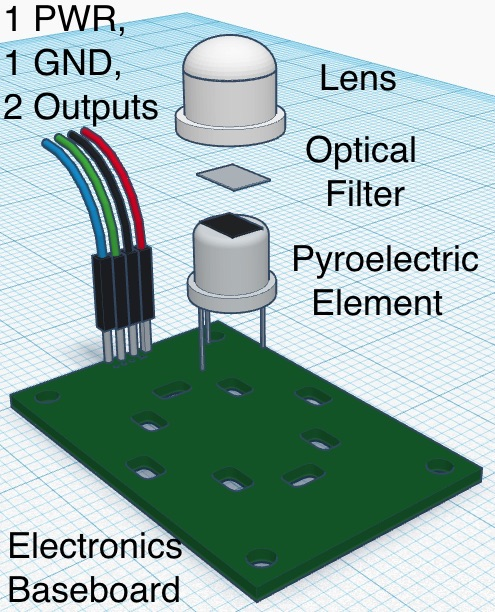
\includegraphics[width=0.2\textwidth, height=1.3in]{figures/platform/3d_view_5-annotated.jpg}
        \caption{PIR Sensor Teardown showing the different subsystems illustrated in TinkerCAD}
        \label{fig:pir_system_teardown}
    %\end{subfigure}%
    % \begin{subfigure}[b]{0.35\textwidth} %\scalebox{0.8}{}
    %     \begin{flushleft}
    %         %\centering
    %         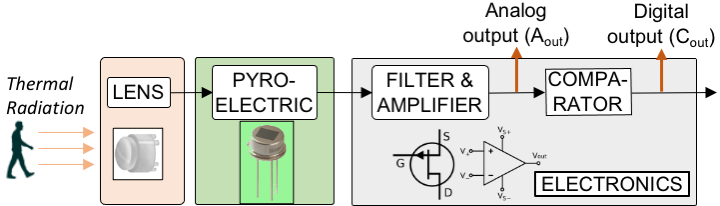
\includegraphics[width=1.2\textwidth]{figures/platform/pir-block-diagram-2-redraw-camera.png}
    %         \caption{}
    %         \label{fig:pir_working}
    %     \end{flushleft}
    % \end{subfigure}%
    %\hfill
    % \begin{subfigure}[b]{0.30\textwidth}
    %     \begin{flushright}
    %     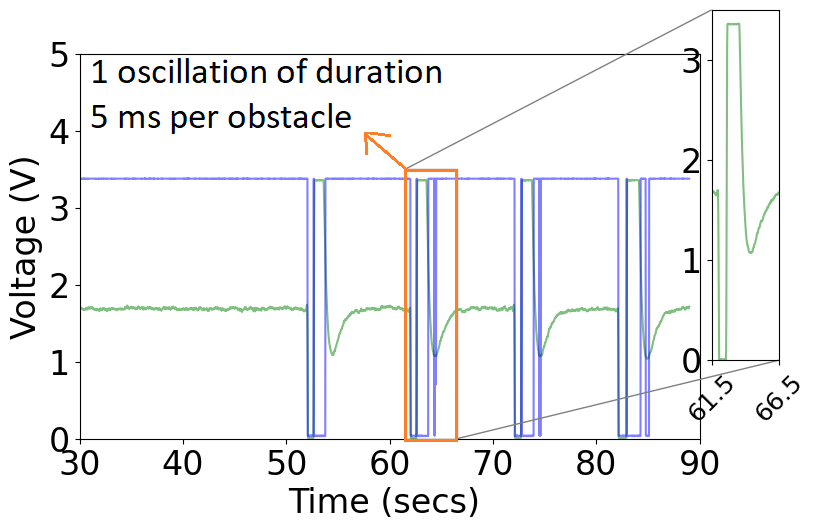
\includegraphics[width=0.9\textwidth]{figures/lens_types/inline_lens.png}
    %     \caption{}
    %     \label{fig:pir_output}
    %     \end{flushright}
    % \end{subfigure}%
    %\caption{\ca \hl{PIR Sensor Teardown}, \cb Internal components of a PIR sensor, \cc Output signals \aout (Green) and \cout (Blue) during sensor operation. \aout, (magnified) shows oscillations when an obstacle is detected}
%\end{figure} 
\end{wrapfigure}

\section{PIR Sensors}
\label{sec:approach}
We take a deep dive into a PIR sensor with 3 goals -- \ca understanding the physics of sensing (\S\ref{subsec:physics}, \S\ref{subsec:working}), \cb correlating physics to the failure scenarios (\S\ref{subsec:taxonomy}) and \cc analyzing the effect of these failures on the sensing performance (\S\ref{subsec:quantify}).

%% BEGINNING OUTLINE
% \begin{itemize}
%     \item Working of the PIR sensor
%     \item Warm behavior - Ashish will email Akshay warmup slides
%     \item Possible faults in PIR sensors - empirical experiments and understanding
%     \item How does $A_{out}$, $C_{out}$ look like for failed scenarios? Plot time domain data and visually show how sensor failure affects $A_{out}$.
% \end{itemize}
%% END OF OUTLINE
%\label{subsec:physics}
%In this section, we briefly describe the working of a PIR sensor and then present the potential failure scenarios in PIR sensors.

\subsection{Background}
\label{subsec:physics}
The teardown of a PIR sensor, showing the internal components is shown in {\bfseries Fig.~\ref{fig:pir_system_teardown}}.
%
%A PIR sensor internally comprises of 3 subsystems as shown in {\bfseries Fig.\ref{fig:pir_working}}  -- \ca a lens, \cb a pyroelectric, and \cc an electronic subsystem. These subsystems act in sequence \ie Lens $\rightarrow$ Pyroelectric $\rightarrow$ Electronic to perform the end-to-end sensing process as we describe next.
It comprises 3 subsystems -- \ca a lens, \cb a pyroelectric attached to an optical filter, and \cc an electronic subsystem.
%
These subsystems act in sequence \ie Lens $\rightarrow$ Pyroelectric $\rightarrow$ Electronic to perform the end-to-end sensing process as shown in {\bfseries Fig.~\ref{fig:pir_sensing_pipeline}}. We describe the different subsystems next.
%

\noindent \underline{\bfseries Lens Subsystem} A plastic fresnel lens~\cite{an_murata} is used to capture and precisely focus thermal radiation into an optical filter that is aimed at a pyroelectric element. 
%The lens is glued to the electronic board via an adhesive and is geometrically constructed to precisely focus thermal radiation on the pyroelectric element. 
Fresnel lenses have a large capture area (aperture) and are used to concentrate radiation into a narrow beam. % and provide a short focal length.
%
They are used to divide the entire region observable to the PIR sensor into small cells, which increases range of the sensor by manifolds. 
%
They have a large capture area (aperture) and are common in a wide variety of applications such as lighthouses, solar cells and even in optical landing systems in aircrafts~\cite{webster1999measurement}.


% \begin{figure*}
% 	%%%%%%%%%%%%%%%%
% 	% PIR SENSOR PIPELINE
% 	%%%%%%%%%%%%%%%%
% 	%\begin{subfigure}{0.48\textwidth}
% 	\begin{minipage}[b]{0.56\linewidth}
% 		%\begin{flushright}
% 		\centering
% 			\begin{subfigure}[t]{\textwidth}
% 				\includegraphics[width=\textwidth,height=0.9in]{figures/platform/pir-block-diagram-2.png}
% 				\caption{}
% 				\label{fig:pir_sensor_pipeline}
% 			\end{subfigure}\\
% 			\begin{subfigure}[t]{\textwidth}
% 				\includegraphics[width=\textwidth,height=0.7in]{figures/platform/sensys_workflow.png}
% 				\caption{}
% 				\label{fig:system_workflow}
% 			\end{subfigure}
% 		%\end{flushright}
% 		\caption{\ca \textbf{Physics of the} PIR Sensing Pipeline, \cb \textbf{End-to-end workflow} of \sol for fault detection and diagnosis.}
% 		\label{fig:pir_sensing_pipeline}
% 	\end{minipage}
% 	%\end{subfigure}%
% 	%%%%%%%%%%%%%%%%
% 	% END OF PIR SENSOR PIPELINE
% 	%%%%%%%%%%%%%%%%
% 	\hspace{5ex}
%     %%%%%%%%%%%%%%%%
%     % PIR Working
%     %%%%%%%%%%%%%%%%
% 	\begin{minipage}[b]{0.39\linewidth}
% 		\centering
% 		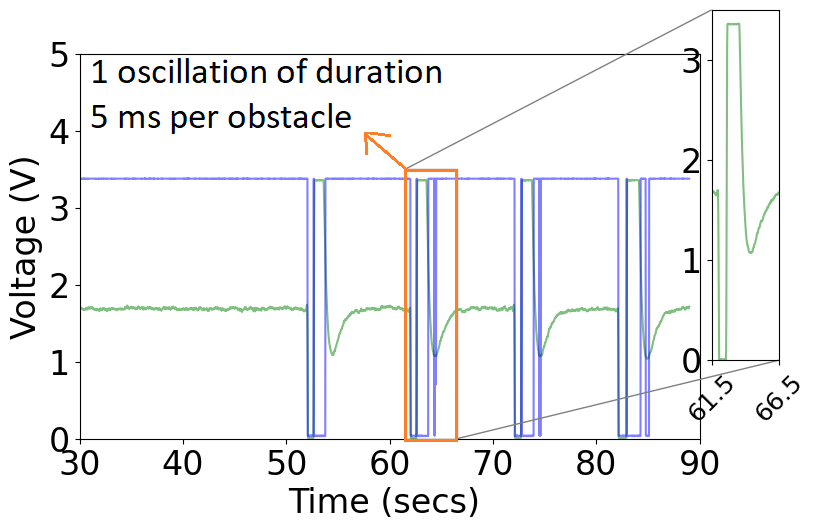
\includegraphics[width=\textwidth]{figures/lens_types/inline_lens.png}
% 		\caption{\textbf{Output signals \aout (Green) and \cout (Blue)} during sensor operation. \aout, (magnified) shows oscillations when an obstacle is detected.}
% 		\label{fig:pir_sensor_working}
% 	\end{minipage}
% 	%%%%%%%%%%%%%%%%
%     % END OF PIR Working
%     %%%%%%%%%%%%%%%%
% \end{figure*}

% Removing PIR Sensor Internals Figure
% \begin{figure*}%{htbp}
% 	%\begin{wrapfigure}{L}{9.5cm}
% 	% \centering
% 	%\vspace{-10pt}
% 	\begin{subfigure}[t]{0.5\textwidth}
% 		\centering
%     	\includegraphics[width=\textwidth]{figures/platform/pir-sensor-internals-2.png}%
%     	\caption{%\st{\textbf{Overview of PIR Sensor Internals} showing various subsystems.}
%     	}
%     	\label{fig:pir_sensor_overview}
% 	\end{subfigure}
% 	%\vspace{-10pt}
% 	%\end{wrapfigure}
% 	\hspace{5ex}
%     %%%%%%%%%%%%%%%%
%     % PIR Working
%     %%%%%%%%%%%%%%%%
% 	\begin{subfigure}[t]{0.4\textwidth}
% 		\centering
% 		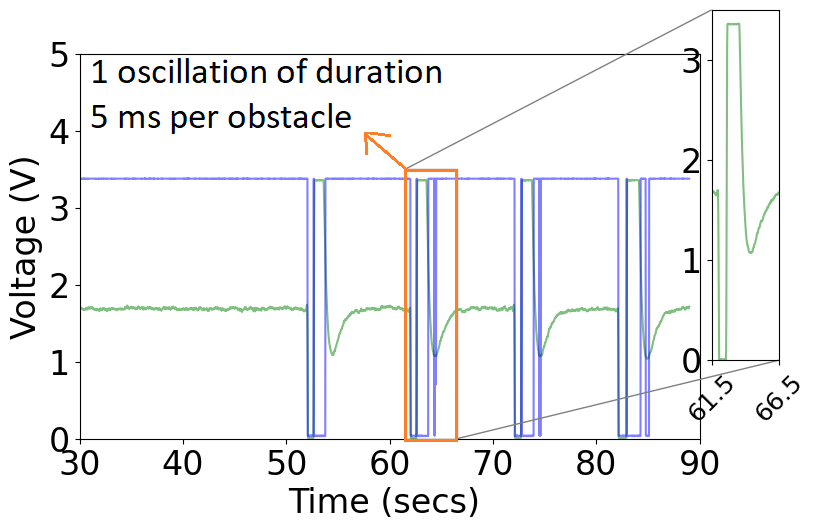
\includegraphics[width=\textwidth]{figures/lens_types/inline_lens.png}
% 		\caption{}
% 		\label{fig:pir_sensor_working}
% 	\end{subfigure}
% 	%%%%%%%%%%%%%%%%
%     % END OF PIR Working
%     %%%%%%%%%%%%%%%%
%     \caption{\ca \textbf{Close-up} of a COTS PIR sensor with its subsystems. \cb \textbf{Output signals \aout (Green) and \cout (Blue)} during sensor operation. \aout, (magnified) shows oscillations when an obstacle is detected.}
% \end{figure*}

\noindent \underline{\bfseries Pyroelectric Subsystem} comprises of an optical filter and a pair of pyroelectric elements. The optical filter is designed to filter out thermal radiations from wavelengths outside the human range (i.e., ~ 5 $\mu$m to 10 $\mu$m), which is then incident on the pyroelectric elements. % ({\bfseries Fig.\ref{fig:pir_system_teardown}}).
The pyroelectric elements convert the thermal radiation into an electrical voltage signal, a process known as the \textit{pyroelectric effect}. The output of the pyroelectric subsystem is an analog signal that is sent to the electronic subsystem.
In practice, there are two pyroelectric elements connected in series in a differential configuration. This differential configuration enables the PIR sensor to detect \textit{movement} of objects as static objects will trigger both the pyroelectric elements equally and cancel out unlike moving objects that trigger both elements unequally resulting in an output from the pyroelectric subsystem. %In other words, with the two pyroelectric elements opposing each other in the sensor, we get a differential voltage at the output of their combination. 
Due to the differential output voltage, the pyroelectric subsystem does not measure the absolute intensity of incident thermal radiation but measures a change in incident thermal radiation, say caused by motion. Note that the pyroelectric element by itself is passive \ie has no power source.

%That is, it produces a potential difference at its two terminals proportional to the incident light.
%This ensures that factors such as ambient room temperature have very less effect on the operation of the sensor.

\noindent \underline{\bfseries Electronic Subsystem} consists of a filter (RC filter), amplifier (JFET or OpAmp) and comparator (OpAmp) circuits. The output from pyroelectric subsystem are filtered to remove noise, amplified to increase its magnitude and finally sent to a comparator to convert analog signals to discrete signals. This \textit{discrete signal is HIGH when there is no motion and goes HIGH$\rightarrow$LOW when motion is detected}. Systems connected to a PIR sensor such as lighting or heating use the discrete signal to regulate the illumination or temperature in a building.

%%%%%%%%%%%%%%%%
% PIR Working
%%%%%%%%%%%%%%%%
% \begin{wrapfigure}{L}{7cm}
% 	% \begin{minipage}[t]{0.49\textwidth}
% 	\centering
% 	%\includegraphics[width=\textwidth, height=1.75in]{figures/pir/working/PIR_EVM_Charac_WithWithoutObstacle-2.png}
% 	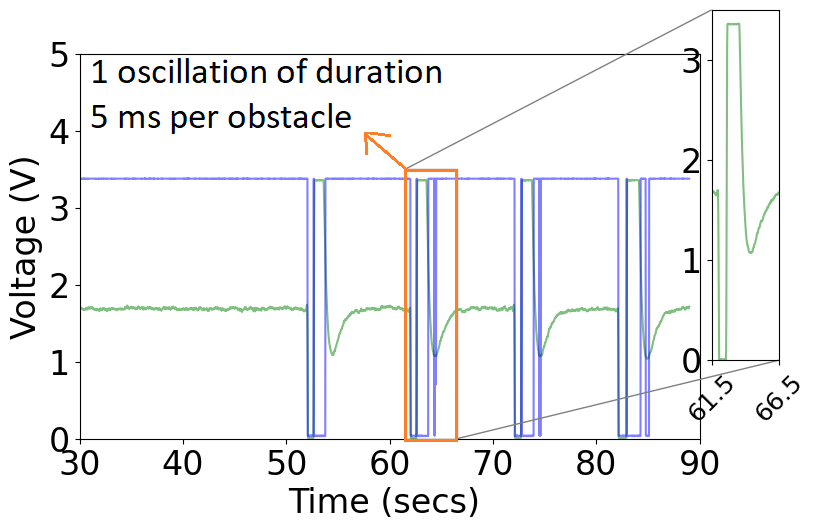
\includegraphics[width=6.5cm]{figures/lens_types/inline_lens.png}
% 	\caption{\textbf{Output signals \aout (Green) and \cout (Blue)} during sensor operation. \aout, drawn magnified shows the oscillations when an obstacle is detected.}
% 	\label{fig:pir_sensor_working}
% 	% \end{minipage}
% \end{wrapfigure}
%%%%%%%%%%%%%%%%
% END OF PIR Working
%%%%%%%%%%%%%%%%

%\subsection{Output Signals of a PIR Sensor}%The final output of the sensor is a discrete voltage signal, referred to as \cout that follows negative logic \ie stays HIGH when there is no motion and goes LOW when motion is detected. 

%The signal from the electronic system before sending it to the comparator is a filtered, amplified version of the output of the output of the pyroelectric subsystem -- this is called \aout.
% The differential voltage is then fed to the gate of a Junction Field-Effect Transistor (JFET). When the JFET is powered, the output at the source of the JFET is controlled by the output of the pyroelectric elements. The construction of the pyroelectric sensor is as shown in Figure. The pyroelectric elements and the JFET are encased in a housing and a filter is placed on top of the pyroelectric elements. This filter allows only infrared light to pass through. A fresnel lens is used to divide the entire region observable to the pyroelectric sensor into small cells. This increases the range of the sensor by manifolds.
% We will now present the working and physics of the PIR sensor.

%\begin{wrapfigure}{L}{0.7\textwidth}
\begin{figure}
	\centering
    \begin{subfigure}[b]{0.4\textwidth} %\scalebox{0.8}{}
        \begin{flushleft}
            %\centering
            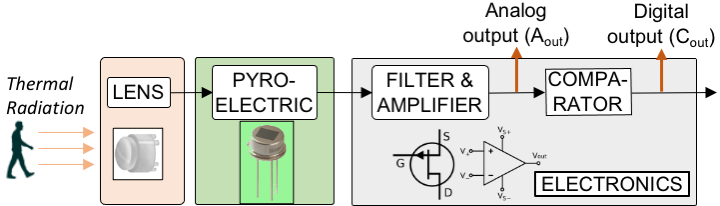
\includegraphics[width=\textwidth]{figures/platform/pir-block-diagram-2-redraw-camera.png}
            \caption{Sensing Pipeline of a PIR Sensor}
            \label{fig:pir_sensing_pipeline}
        \end{flushleft}
    \end{subfigure}%
    \hfill
	\begin{subfigure}[t]{0.3\textwidth}
		\centering
		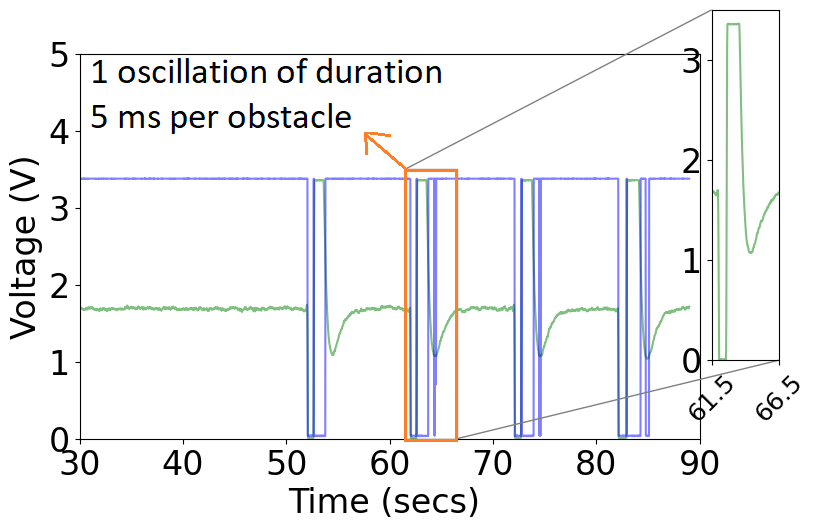
\includegraphics[width=\textwidth]{figures/lens_types/inline_lens.png}
		\caption{Inline lens (wall-mount)}
		\label{fig:inline_lens}
	\end{subfigure}%
    %\hspace{1ex}
	\begin{subfigure}[t]{0.3\textwidth}
		\centering
		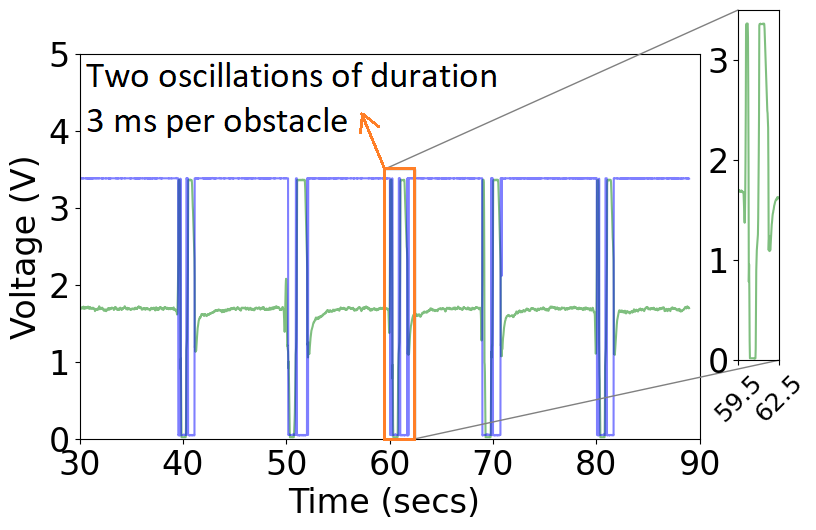
\includegraphics[width=\textwidth]{figures/lens_types/round_lens.png}
		\caption{Round lens (ceiling-mount)}
		\label{fig:round_lens}
	\end{subfigure}	   
	\caption{Effect of different types of lens on the \aout curve, shown in green -- the inline lens type produces a single oscillation whereas a round lens type produces two oscillation per obstacle. The corresponding \cout, shown in blue, stays HIGH when there is no motion and goes LOW when motion is detected. }
	\label{fig:pir_sensor_different_lens}
\end{figure}
%\end{wrapfigure}

\subsection{\textbf{Analysis of Output Signals of a PIR Sensor:}}
\label{subsec:working} 
There are 2 output signals from a PIR sensor as shown in {\bfseries Fig.~\ref{fig:pir_sensing_pipeline}}:
% \vspace{-5pt}
\begin{enumerate} \item \textbf{Final discrete output} of the electronic subsystem (\cout) that follows negative logic \ie stays HIGH when there is no motion and goes LOW when motion is detected. \item \textbf{Intermediate analog output} just prior to the discretization process (\aout). \end{enumerate}

%We consider the 2 output signals of the sensor -- \ci The Output from the Electronics (\cout) and \cii The Output from the Pyroelectric Element (\aout).  
To analyze \cout and \aout during operation, we interface a PIR sensor to an Arduino microcontroller~\cite{arduino_mega}. 
% This is plotted in \textbf{Fig.~\ref{fig:pir_sensor_working}} for a period of 60 seconds.
{\bfseries Fig.~\ref{fig:inline_lens} --~\ref{fig:round_lens}} shows plots of \aout and \cout for a period of 60 seconds, both in the presence and absence of an obstacle. The y-axis represents voltages seen at the output and x-axis represents time. As expected, %the discrete signal 
\cout, marked in blue, goes LOW when an obstacle comes into the field of view %(\ie there is motion) 
and stays HIGH otherwise. On the other hand, %the analog signal 
\aout, marked in green, measures around 1.8 V when there is no obstacle and produces oscillation(s) when an obstacle comes into the field of view (shown magnified). 
%
The nature and shape of the \aout curve also depends on the nature of lens used in the PIR sensor. Typically, an inline lens is used for the wall-mount version and a round lens is used for the ceiling-mount version. {\bfseries Fig.~\ref{fig:pir_sensor_different_lens}} also shows the variations in \aout between the two lens types -- \ca Inline lens has a wider curve compared to round lens and \cb Round lens has double number of oscillations of \aout curve per obstacle. We used a wall-mount PIR sensor in our experiments though our analysis, techniques and observations are equally applicable to ceiling-mount sensors. %sensing performance. 
%
With a working background on PIR sensors, we next study the various failures in a PIR sensor and its impact on sensing physics.